\documentclass[border=4pt]{standalone}
\usepackage{fontspec}
\usepackage{amsmath}
\usepackage{unicode-math}
\setmainfont{Latin Modern Roman}
\setmathfont{Latin Modern Math}
\usepackage{pgfplots}
\usepackage{pgfplotstable}
\pgfplotsset{compat=1.18}
\usepackage{tkz-euclide}
\usetikzlibrary{arrows.meta,calc,angles,quotes,patterns,3d,backgrounds}
\definecolor{ink}{HTML}{123428}
\definecolor{asy}{HTML}{475569}
\definecolor{mint}{HTML}{86e0bd}
\tikzset{asym/.style={asy, line width=0.9pt, dash pattern=on 5pt off 3.5pt},
         guide/.style={gray!70, line width=0.6pt, densely dotted},
         dot/.style={circle, inner sep=0pt, minimum size=5pt, draw=white, line width=0.5pt},
         odot/.style={circle, inner sep=0pt, minimum size=5.5pt, fill=white, line width=1pt},
         lab/.style={font=\footnotesize, inner sep=1.5pt, text=ink}}
\begin{document}
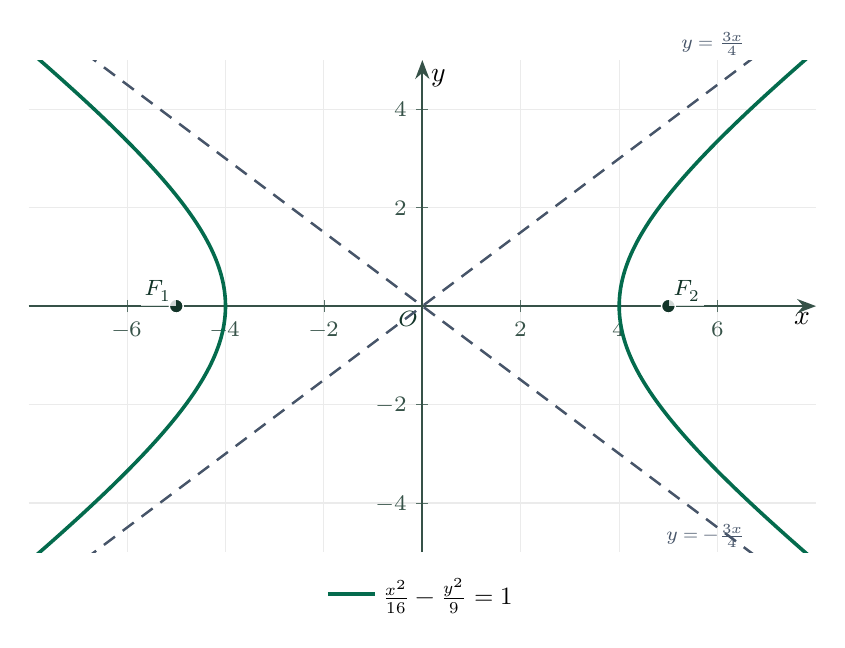
\begin{tikzpicture}
\begin{axis}[
  scale only axis,
  width=10.00cm,
  height=6.25cm,
  axis lines=middle,
  xmin=-8, xmax=8, ymin=-5, ymax=5,
  axis line style={draw=ink!85, line width=0.7pt, -{Stealth[length=2.4mm]}},
  xlabel={$x$}, ylabel={$y$},
  xlabel style={at={(ticklabel* cs:1)}, anchor=north east, inner sep=2pt},
  ylabel style={at={(ticklabel* cs:1)}, anchor=north west, inner sep=3pt},
  grid=major, major grid style={draw=gray!16, line width=0.4pt},
  tick style={draw=ink!70},
  ticklabel style={font=\footnotesize, text=ink!85},
  xtick={-6,-4,-2,2,4,6},
  xticklabels={$-6$,$-4$,$-2$,$2$,$4$,$6$},
  ytick={-4,-2,2,4},
  yticklabels={$-4$,$-2$,$2$,$4$},
  clip mode=individual,
  every axis plot/.append style={line join=round},
  legend style={at={(0.5,-0.03)}, anchor=north, draw=none, fill=none, font=\small, legend columns=-1, /tikz/every even column/.append style={column sep=10pt}},
  legend cell align=left]
\node[lab, anchor=north east] at (axis cs:0,0) {$O$};
\addplot[asym, draw={rgb,255:red,71;green,85;blue,105}, forget plot, domain=-8:8, samples=2] {0.75*x+(0)};
\node[lab, text=asy, anchor=south east, font=\scriptsize] at (axis cs:6.666667,5) {$y = \frac{3x}{4}$};
\addplot[asym, draw={rgb,255:red,71;green,85;blue,105}, forget plot, domain=-8:8, samples=2] {-0.75*x+(0)};
\node[lab, text=asy, anchor=south east, font=\scriptsize] at (axis cs:6.666667,-5) {$y = -\frac{3x}{4}$};
\addplot[color={rgb,255:red,4;green,107;blue,77}, line width=1.3pt, variable=\t, domain=-1.75:1.75, samples=160, smooth] ({4*cosh(\t)},{3*sinh(\t)});
\addlegendentry{$\frac{x^{2}}{16} - \frac{y^{2}}{9} = 1$}
\addplot[color={rgb,255:red,4;green,107;blue,77}, line width=1.3pt, variable=\t, domain=-1.75:1.75, samples=160, smooth, forget plot] ({-4*cosh(\t)},{3*sinh(\t)});
\node[dot, fill={rgb,255:red,18;green,52;blue,40}] at (axis cs:-5,0) {};
\node[lab, anchor=south east, fill=white, fill opacity=0.8, text opacity=1] at (axis cs:-5,0) {$F_{1}$};
\node[dot, fill={rgb,255:red,18;green,52;blue,40}] at (axis cs:5,0) {};
\node[lab, anchor=south west, fill=white, fill opacity=0.8, text opacity=1] at (axis cs:5,0) {$F_{2}$};
\end{axis}
\end{tikzpicture}
\end{document}
